\documentclass[10pt]{article}
\usepackage[a4paper,margin=16mm]{geometry}
\usepackage[T1]{fontenc}
\usepackage{lmodern,microtype,graphicx,booktabs,tabularx,xcolor,hyperref,caption,enumitem,titlesec,float}
\definecolor{jepablue}{HTML}{2A6FBB}
\definecolor{warningred}{HTML}{B3261E}
\definecolor{softgray}{HTML}{F3F5F7}
\hypersetup{colorlinks=true,linkcolor=jepablue,urlcolor=jepablue}
\captionsetup{font=small,labelfont=bf}
\setlist{nosep,leftmargin=5mm}
\setlength{\parindent}{0pt}
\setlength{\parskip}{4pt}
\titleformat{\section}{\large\bfseries\color{jepablue}}{}{0pt}{}
\graphicspath{{figures/}}
\title{\vspace{-10mm}\textbf{Intent-Phrase JEPA for Planning}\\[-1mm]\large Current evidence, failed scaling gate, and next decisions}
\author{TextJEPA research summary}
\date{4 August 2026}

\begin{document}
\maketitle\vspace{-6mm}
\begin{center}
\fcolorbox{jepablue}{softgray}{\parbox{0.91\linewidth}{\textbf{Bottom line.} Joint-Embedding Predictive Architecture (JEPA) models plan competitively in a controlled language-action world and geometric advantage ranking (GAR) is essential. The sentence-plus-latent baseline still leads strict success; a direct ranker currently matches JEPA on one seed; and the first apparent deep-planning curve is invalid because symbolic candidate generation exposes short terminal paths.}}
\end{center}

\section{Question and setting}
Think of each puzzle as a locked room and each intent phrase as an action card. A language model asks which card text is likely next. A JEPA instead predicts how its internal state changes after each card and uses GAR to order promising and unpromising consequences. We ask whether this predictive geometry is a viable and analyzable basis for planning---not whether a toy model beats state of the art.

Headline systems train on 300,000 freshly generated stylized-iGSM examples with 3--9 necessary actions. At each environment step, every model receives the same prompt, observed history, and symbolic menu of currently feasible action phrases. Strict success permits no detour; $+2$ permits two excess actions. Main and ablation results use five seeds and 200 fresh validation puzzles per seed.

\section{Headline result: viable, competitive, not superior}
\begin{table}[H]
\centering\small
\begin{tabular}{lccc}\toprule
Model & Strict & $+2$ actions & Seeds \\\midrule
Sentence LM + latent loss & $\mathbf{.521\pm.047}$ & $.809\pm.020$ & 5\\
Sentence LM & $.471\pm.046$ & $.813\pm.023$ & 5\\
MLP JEPA & $.433\pm.019$ & $.796\pm.033$ & 5\\
Token LM & $.422\pm.124$ & $\mathbf{.836\pm.073}$ & 5\\
Causal JEPA & $.366\pm.047$ & $.778\pm.043$ & 5\\\bottomrule
\end{tabular}
\caption{Mean $\pm$ sample standard deviation over training seeds. MLP JEPA is competitive and stable, but the generative-plus-latent hybrid is the strict leader.}
\end{table}
\begin{figure}[H]\centering
\includegraphics[width=.94\linewidth]{headline_models.pdf}
\caption{All systems use the same currently feasible action menu. This is a controlled candidate interface, not unrestricted generation.}\end{figure}

\section{GAR is the supported architectural contribution}
Removing GAR collapses strict success from $.433$ to $.076$; latent-MSE-only reaches $.183$. Ranking-only ($.358$) and no-counterfactual-latent ($.345$) both lose substantial accuracy. Horizon two is much better than horizons one ($.161$) and four ($.181$) under the current random-continuation target. Four counterfactual alternatives improve only modestly over one ($.439$ versus $.403$).
\begin{figure}[H]\centering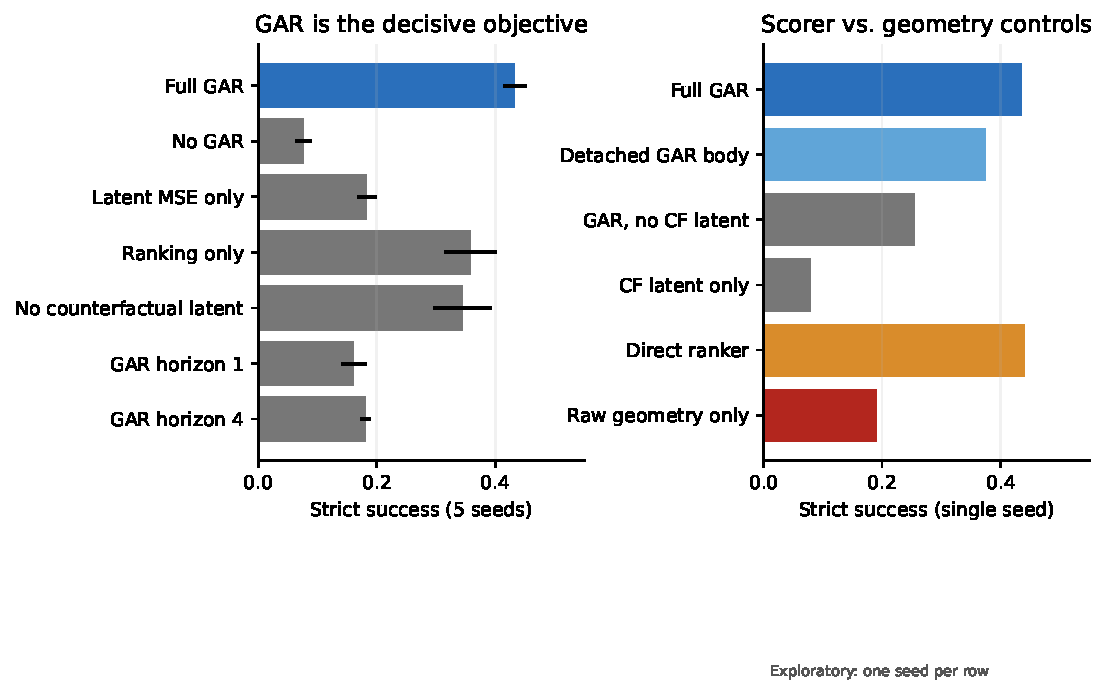
\includegraphics[width=.97\linewidth]{gar_mechanism.pdf}
\caption{\textbf{Left:} five-seed objective ablations. \textbf{Right:} one-seed mechanism controls. A direct ranker matches full JEPA in-distribution; raw metric geometry is weak.}\end{figure}
The 500-episode decision audit localizes the mechanism. The deployed predicted-transition value reaches $.786$ competitive top-1 optimal-action recall and $.826$ pairwise accuracy. Raw predicted geometry reaches only $.549$ and $.603$. GAR currently produces a useful local decision surface more clearly than a globally useful Euclidean goal metric.

\section{What the representations contain}
\begin{figure}[H]\centering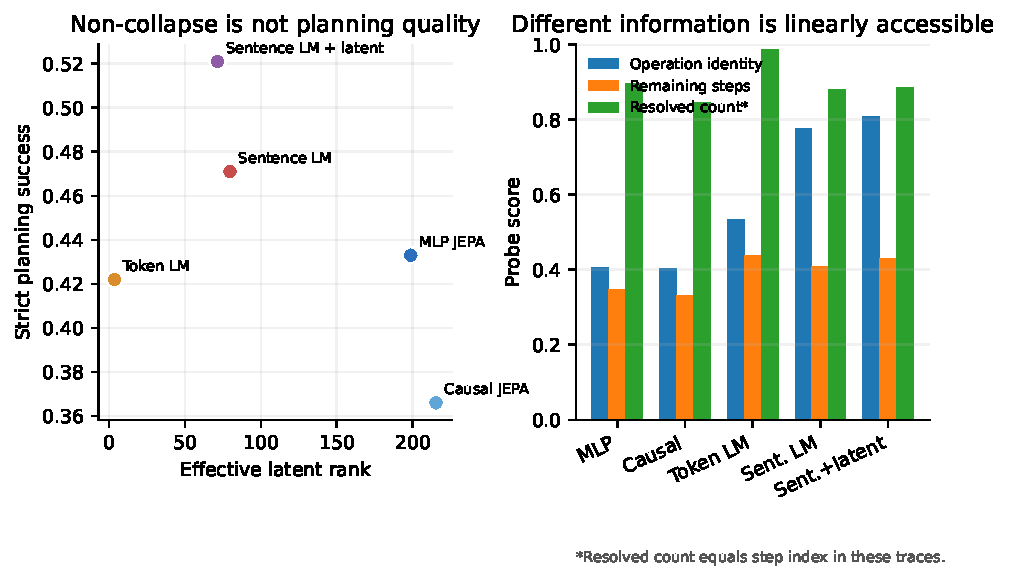
\includegraphics[width=.97\linewidth]{representation_diagnostics.pdf}
\caption{High rank establishes non-collapse, not planning quality. Sentence models expose operation identity more linearly. Resolved count is highly decodable but equals elapsed step index in these traces.}\end{figure}
MLP JEPA has effective rank $198.7$, remaining-step $R^2=.346$, and resolved-count $R^2=.895$. Sentence-plus-latent states have effective rank $71.4$ but operation balanced accuracy $.808$, versus $.406$ for MLP JEPA. Numerical outcomes are weakly decoded across systems. The necessary-action probe is invalid as positive evidence: balanced accuracy is chance ($.500$).

\section{Test-time compute: one real result and one failed gate}
\begin{figure}[H]\centering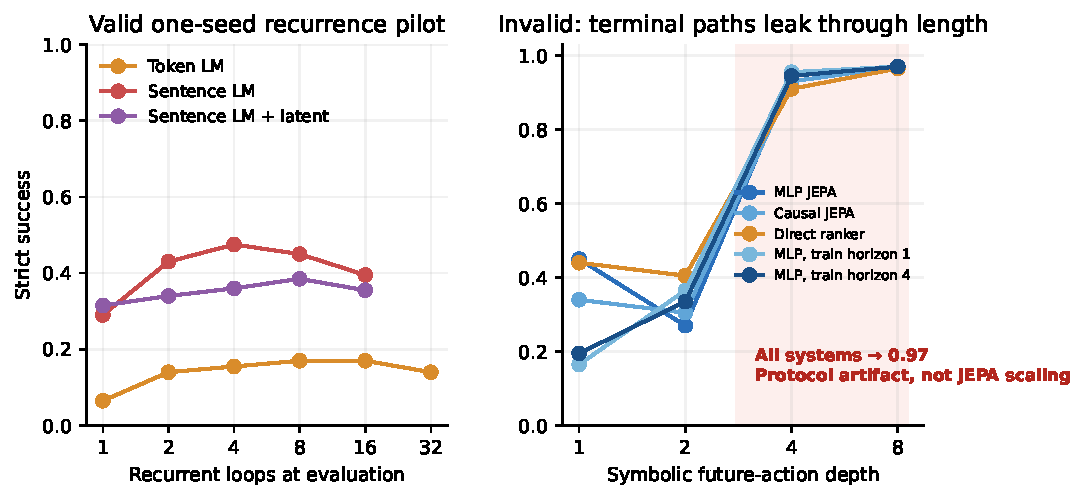
\includegraphics[width=.98\linewidth]{test_time_compute.pdf}
\caption{\textbf{Left:} Poisson-trained recurrent language models improve and then overthink (one seed). \textbf{Right:} the fixed-checkpoint JEPA pilot is scientifically invalid: all architectures approach $.97$ because terminal paths are returned early and favored by path length.}\end{figure}
The recurrent sentence LM rises from $.290$ at one loop to $.475$ at four loops, then falls to $.395$ at sixteen. The token model rises from $.065$ to about $.170$. These are legitimate one-seed accuracy curves, although current FLOP tracing barely changes with loop count and must be repaired before compute-matched claims.

The fixed-checkpoint latent-lookahead jobs all completed and checkpoint hashes match. However, the reference enumerator returns a sequence as soon as it contains the query, while the energy adds sequence length. At depths four and eight, JEPA, causal JEPA, and the direct ranker all jump to $.91$--$.97$. This convergence is an interface leak, not evidence that latent simulation scales.

\section{Length generalization remains open}
\begin{figure}[H]\centering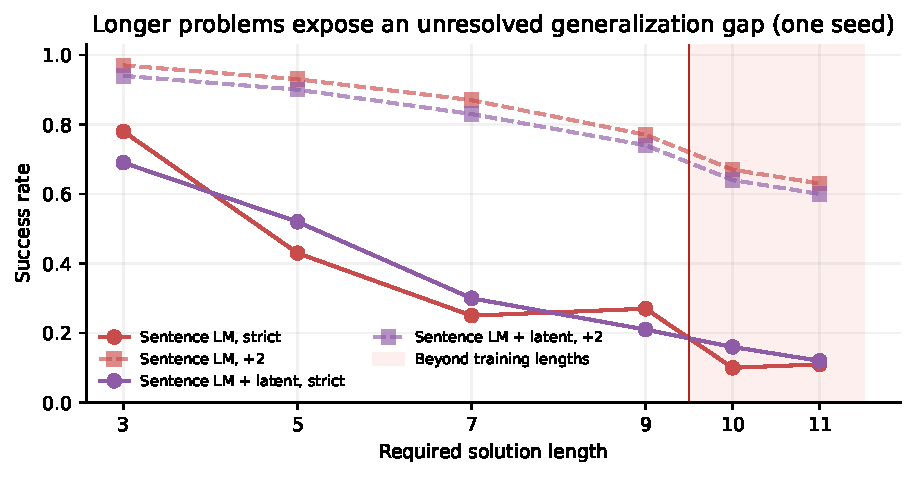
\includegraphics[width=.86\linewidth]{length_ood.pdf}
\caption{Distractor-matched exact-length evaluation for two sentence families (one seed, 100 puzzles per cell). Both degrade beyond the 3--9 training range.}\end{figure}
At strict evaluation, the sentence LM falls from $.27$ at length nine to $.10/.11$ at lengths ten/eleven; sentence-plus-latent falls from $.21$ to $.16/.12$. Full JEPA and token curves and multi-seed confirmation are still missing.

\section{Claims, limitations, and next decisions}
\textbf{Supported now}
\begin{itemize}
\item A non-generative JEPA can perform competitive closed-loop language-action planning.
\item GAR, counterfactual latent prediction, and direct advantage regression form the central useful mechanism.
\item JEPA is high-rank and exposes progress variables, while generative sentence states expose operation identity better.
\item Recurrent generative computation helps up to an intermediate loop count.
\end{itemize}
\textbf{Not supported now}
\begin{itemize}
\item JEPA superiority over sentence models, direct ranking, or compute-matched baselines.
\item Deep JEPA test-time scaling under the current symbolic future-action protocol.
\item A claim that global latent distance alone supplies planning geometry.
\item Broad language reasoning, robust length OOD, or paraphrase/negation invariance.
\end{itemize}
\textbf{Next experiments, in order}
\begin{enumerate}
\item Repair scaling: fixed-length candidates, no early-terminal return, absorbing padding after solve, no path-length preference, randomized order, and shuffled/untrained-score controls.
\item Repeat a one-seed gate with MLP JEPA and direct ranker at depths $\{1,2,4\}$ on 1,000 paired puzzles. Scale only if controls stay flat and JEPA improves.
\item Run five seeds for the direct ranker and detached-GAR-body control; correlate ranking accuracy, margin, regret, drift, MSE, rank, and strict success.
\item Test predictive factorization on data efficiency, longer compositions, paraphrases, negations, entity renaming, and novel goals.
\item Repair recurrent FLOP accounting; compare paired success versus verified FLOPs; add shared generative proposals plus JEPA reranking as the non-oracle scaling result.
\item Add one small second language-action domain after the mechanism gate passes.
\end{enumerate}

\section{Reproducibility}
All plots are generated from controller-retrieved artifacts by \href{run:make_figures.py}{\texttt{make\_figures.py}}; extracted values are in \href{run:report_data.json}{\texttt{report\_data.json}}. The test-time round is \texttt{2026-08-04-intent-fixed-checkpoint-ttc-pilot-v1}. Candidate-privileged, oracle, single-seed, invalid, and post-evaluation process-failure evidence is labeled rather than silently discarded.
\end{document}
